\begin{frame}[allowframebreaks]{DiffusionPDE}
    % \frametitle{Diffusion Partial Differential Equation (PDE)}

    The diffusion equation is a fundamental PDE describing the distribution of a quantity (such as heat or particles) diffusing through a medium:
    \begin{equation}
        \frac{\partial u}{\partial t} = D \nabla^2 u
    \end{equation}
    where:
    \begin{itemize}
        \item $u = u(\mathbf{x}, t)$ is the quantity of interest (e.g., concentration, temperature)
        \item $D$ is the diffusion coefficient
        \item $\nabla^2$ is the Laplacian operator
    \end{itemize}

    \framebreak

    \begin{figure}
        \centering
        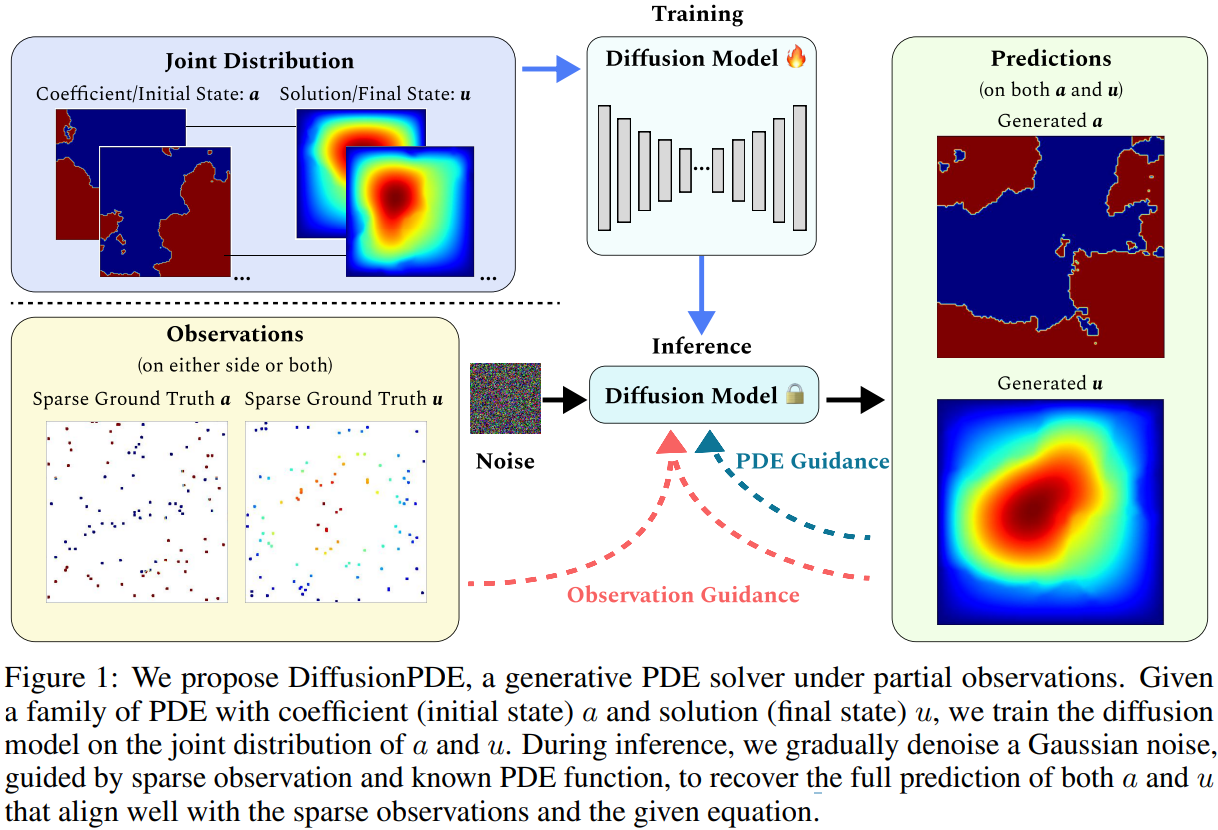
\includegraphics[width=\linewidth,height=\textheight,keepaspectratio]{images/adv-img-gen/diffusionpde-1.png}
    \end{figure}

    \framebreak

    \begin{figure}
        \centering
        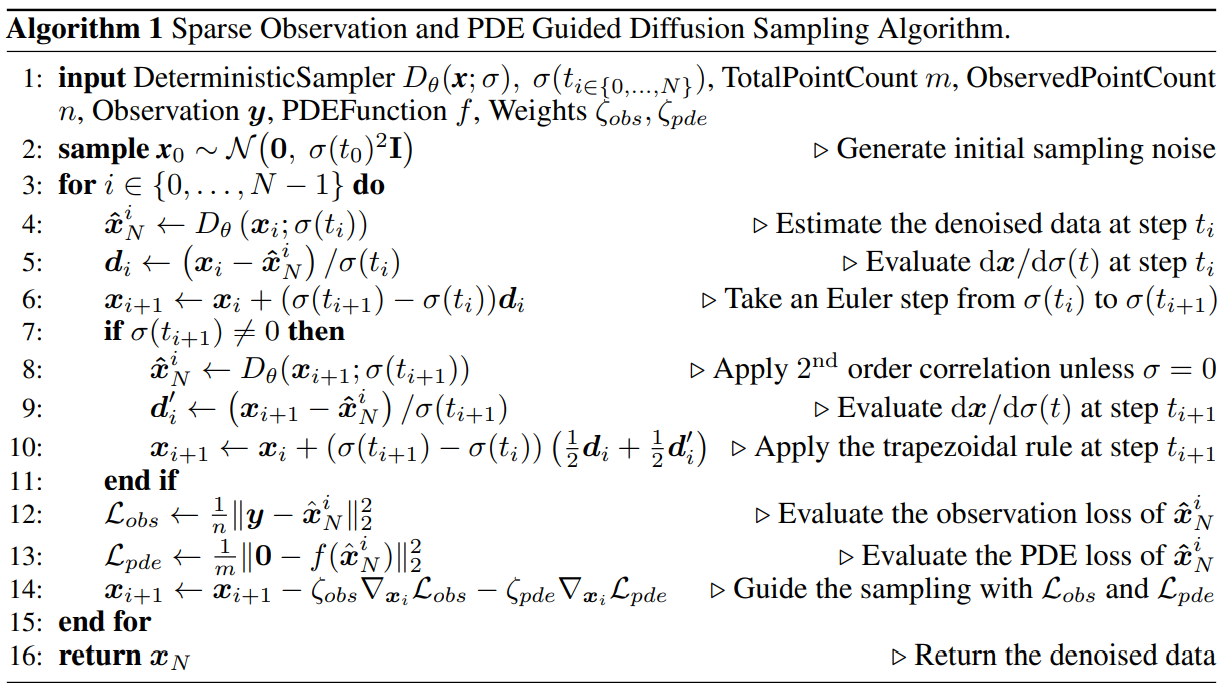
\includegraphics[width=\linewidth,height=\textheight,keepaspectratio]{images/adv-img-gen/diffusionpde-algo-1.png}
    \end{figure}

    \framebreak

    \begin{figure}
        \centering
        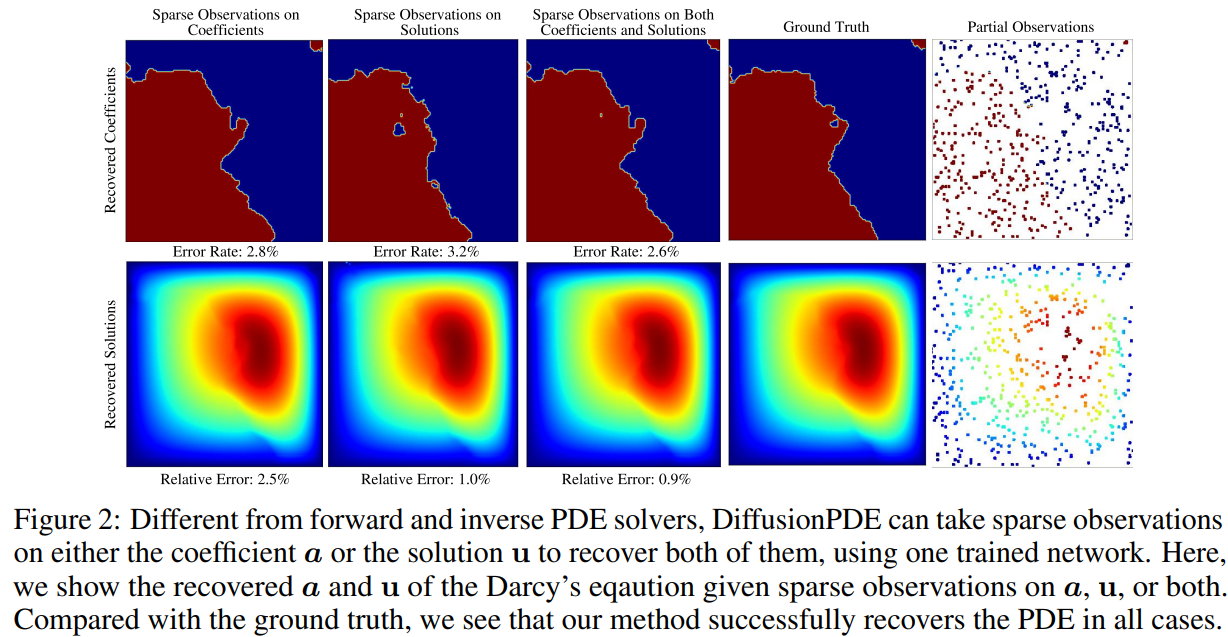
\includegraphics[width=\linewidth,height=\textheight,keepaspectratio]{images/adv-img-gen/diffusionpde-2.png}
    \end{figure}

    \framebreak

    \begin{figure}
        \centering
        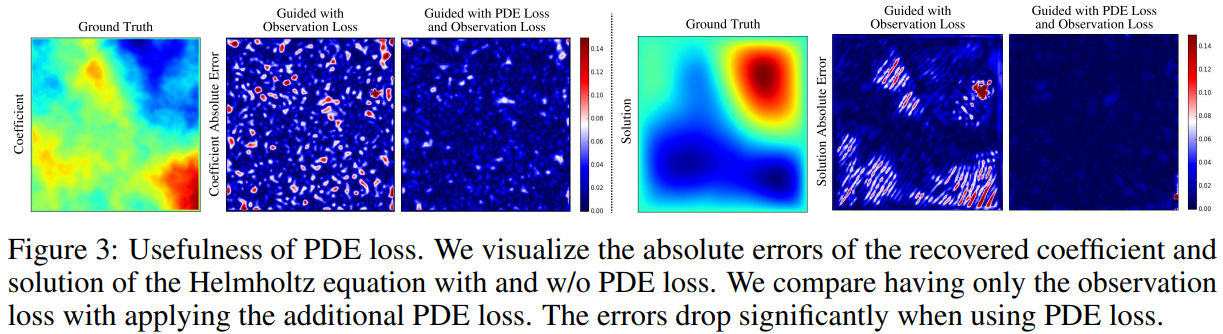
\includegraphics[width=\linewidth,height=\textheight,keepaspectratio]{images/adv-img-gen/diffusionpde-3.png}
    \end{figure}
\end{frame}